\chapter{Wyniki oceny eksperymentalnej}

\noindent W tej sekcji zostaną przedstawione oceny predykcji wyników meczy piłkarskich osiągnięte na danych testowych przez wybrane algorytmy uczące się wchodzące w skład systemu. 

Chcemy przypomnieć, że sport, jakim jest piłka nożna, należy do dyscyplin bardzo złożonych, charakteryzujących się ogromną liczbą zmiennych, które są słabo przewidywalne i trudne do uwzględnienia. Ponadto w rzeczywistości wynik predykcji meczu  determinowany jest pewną dozą szczęścia dla jednej z drużyn. Inne czynniki są również trudne do uwzględnienia. Warunki pogodowe, dyspozycja danego zawodnika oraz nastawienie każdego z graczy jest często czynnikiem kluczowym, lecz niestety niemożliwym do uchwycenia w przypadku typowych danych historycznych, a tym bardziej w celu wykorzystania do predykcji wyniku spotkania. Jednak istnieją również czynniki reprezentowane przez atrybuty, które mają realny wpływ na wynik i właśnie je postarano się w tej pracy zidentyfikować, uwzględnić oraz na ich podstawie dokonywać obliczeń i zwracać rezultaty o potencjalnym zwycięzcy. Dane przygotowane i przetworzone (patrz opis w poprzednich rozdziałach) były podstawą do osiągnięcia wyników naszego systemu, które przedstawiono w poszczególnych podsekcjach dla wybranych algorytmów. 

W posiadanych danych występują 3 następujące klasy, które trzeba przewidzieć: 
\begin{itemize}
    \item \english{Draw} - oznacza remis pomiędzy drużynami (etykieta 0)
    \item \english{HomeWin} - oznacza, że drużyna definiowana jako gospodarz odniosła zwycięstwo (etykieta 1)
    \item \english{AwayWin} - oznacza, że drużyna definiowana jako gość odniosła zwycięstwo (etykieta 2)
\end{itemize}

Liczba przykładów z poszczególnych klas w zbiorze danych przed operacją odlosowania przedstawiono w tabeli \ref{tab:przedOdlosowaniem} 

\begin{table}[H]
    \centering
    \caption{Liczba przykładów  w poszczególnych klasach przed odlosowaniem}
    \label{tab:przedOdlosowaniem}
    \begin{tabular}{| c  c |}
    \hline
         Draw & 586 \\
         HomeWin & 1021 \\
         AwayWin & 662 \\\hline
    \end{tabular}
\end{table}
Jak widać, klasa oznaczająca wygraną drużyny gospodarzy, posiada prawie dwukrotnie więcej przykładów niż pozostałe klasy. Dlatego powyższy zbiór danych został zmniejszony w taki sposób, że najliczniejsza klasa została w przybliżeniu wyrównana do klasy mniej licznej uzyskując w ten sposób bardziej zbalansowane dane, w których nie ma jednej, bardzo dominującej klasy. Metoda wykorzystana do zmniejszenia danych to losowe usunięcie elementów z klasy najbardziej licznej (odpowiednik metod z grupy \english{undersampling}) i właśnie taki zbiór został wykorzystany w dalszym etapie algorytmów (wyniki operacji można zaobserwować w tabeli \ref{tab:poOdlosowaniu}). 

\begin{table}[H]
    \centering
    \caption{Liczba przykładów w poszczególnych klasach po odlosowaniu}
    \label{tab:poOdlosowaniu}
    \begin{tabular}{| c  c |}
    \hline
         Draw & 586 \\
         HomeWin & 662 \\
         AwayWin & 662 \\\hline
    \end{tabular}
\end{table}
Kolejnym krokiem było przygotowanie odpowiednich zbiorów (testowy, walidacyjny oraz treningowy) i rozkład poszczególnych klas w tych zbiorach można zobaczyć w tabeli \ref{tab:rozkłądDanych}.

\begin{table}[H]
\caption{Rozkład danych w odpowiednich zbiorach}
\label{tab:rozkłądDanych}
\centering
\begin{tabular}{| c | c c c |}
\hline
    Klasa & zbiór treningowy & zbiór walidacyjny & zbiór testowy \\ \hline
   Draw & 489 & 32 & 65 \\
   HomeWin & 572 & 31 & 59  \\
   AwayWin & 562 & 33 & 67 \\ \hline
\end{tabular}
\end{table}


We wszystkich algorytmach próbowano również sposobu na nadlosowanie przykładów uczących metodą GlobalCS \cite{GlobalCS} i niestety w każdym z algorytmów rezultaty na wartości trafności (\english{accuracy}) były niższe, dlatego zrezygnowano z tej techniki.

\section{Sztuczne sieci neuronowe}
\label{SNN-results}
\noindent W tej podsekcji, przedstawione zostaną wyniki, które udało się osiągnąć dla struktury sztucznej sieci neuronowej, której parametry wraz z opisem zostały przedstawione w sekcji \ref{SNN-opis} oraz \ref{SNN-param}. Ogólna dokładność - trafność predykcji (\english{accuracy}), obliczona na zbiorze testowym, stanowiącym 10\% z dostępnego zbioru danych wyniosła \definicja{50.79\%}, co w ogólności jest wynikiem satysfakcjonującym, ponieważ w chwili w której osoba zainteresowana predykcją zgadywała by wynik spotkania z równym prawdopodobieństwem wystąpienia jednego z trzech rezultatów, średnia trafność wyniosłaby około 33\%, tak więc wartość powyżej tej liczby jest czymś więcej niż opcją zwykłego zgadywania wyniku. Ponadto inne algorytmy nie doprowadzały do dokładności radykalnie wyższych. 

Wartości innych miar przedstawiono w tabeli \ref{tab:SNNscore}.

\begin{table}[H]
    \centering
    \caption{Wyliczone średnie wartości miar klasyfikacyjnych dla SNN}
    \label{tab:SNNscore}
    \begin{tabular}{| c | c |}
    \hline
         Precyzja (\english{precision}) &  50.41\%\\
         \hline
         Czułość (\english{recall}) &  51.06\%\\
         \hline
         Wartość Fscore &  49.78\%\\
         \hline
    \end{tabular}
\end{table}


Przypomnijmy że miarę precyzji można interpretować jako stosunek $\frac{tp}{tp + fp}$, gdzie tp to liczba poprawnie sklasyfikowanych przykładów, a fp to liczba niepoprawnie sklasyfikowanych przykładów negatywnych jako klasy pozytywnej. Czułość z kolei można interpretować jako stosunek $\frac{tp}{tp + fn}$, gdzie tp jest liczbą poprawnie sklasyfikowanych przykładów pozytywnych, a fn liczba niepoprawnie sklasyfikowanych przykładów pozytywnych jako predykcji w klasie negatywnej -- czyli jest to lokalna dokładność rozpoznania klasy. Fscore interpretuje się jako ważoną średnią harmoniczną precyzji i czułości. Dodatkowo, warto zaznaczyć, że miary te są obliczane na podstawie nieważonej średniej poszczególnych wyników z tych miar i właśnie dlatego, tabela \ref{tab:SNNscore} zawiera pojedyncze wartości takich średnich po klasach. 
Macierz pomyłek przedstawia się następująco:

\begin{center}
\begin{table}[H]
\renewcommand{\arraystretch}{1.5}
\caption{Macierz pomyłek dla SNN}
\label{tab:macierzSNN}
\begin{center}
\begin{tabular}{|c|c|c|c|c|}
   \cline{3-5} 
   \multicolumn{1}{c}{} & & \multicolumn{3}{c|}{Predicted} \\ \cline{3-5}
   \multicolumn{1}{c}{} & & Draw & HomeWin & AwayWin \\ \hline
   
   {Observed/actual}
   & Draw & 20 & 23 & 22 \\ \cline{2-5}
   & HomeWin & 12 & 37 & 10  \\ \cline{2-5}
   & AwayWin & 10 & 17 & 40 \\ \hline
\end{tabular}
\end{center}
\end{table}
\end{center}


Można zauważyć, że najwięcej błędów popełnianych w predykcji, jest w momencie, kiedy faktyczna klasa symbolizuje remis pomiędzy drużynami. 

Po procesie nauki sieci postanowiono dodatkowo sprawdzić wpływ danych cech wejściowych na predykcję danego wyniku i odkryć, które atrybuty odgrywały kluczowe role dla predykcji konkretnego wyniku. Dokonaliśmy tego przy użyciu wartości Shapleya \cite{shapley} oraz biblioteki w języku Python \definicja{Shap}.
\begin{figure}[H] 
        \centering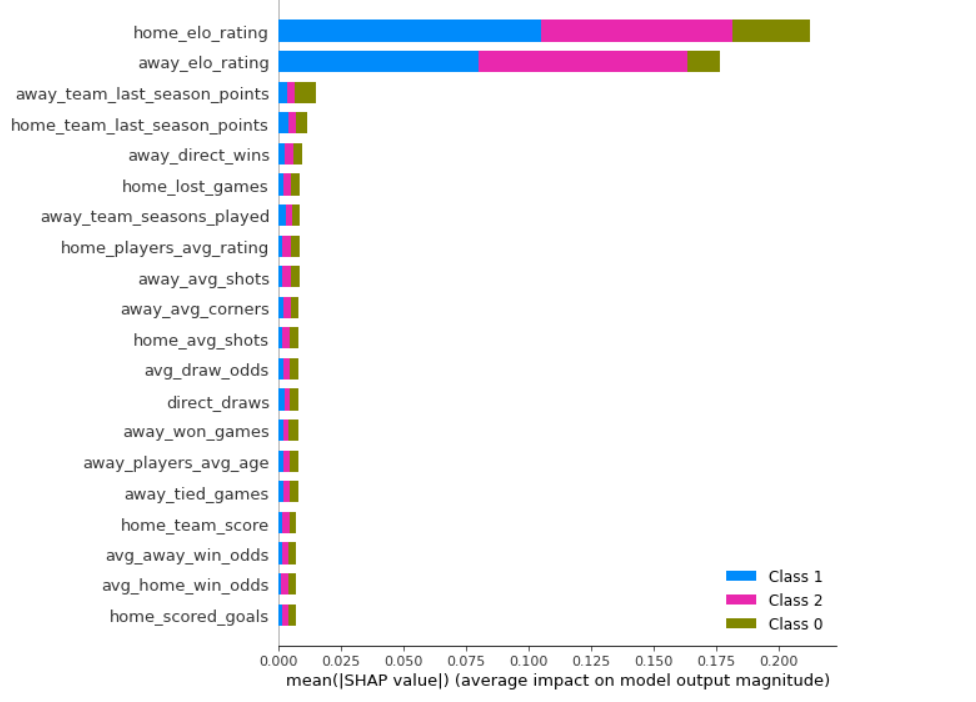
\includegraphics[width=10cm,height=6cm]{figures/ShapSNN.png}
        \caption{Wartości Shapleya dla SNN}\label{Shap-SNN}
\end{figure}

Jak można zauważyć na rysunku \ref{Shap-SNN}, atrybut \textit{home\_elo\_rating} oraz \textit{away\_elo\_rating} miały największe znaczenie (wartość Shapleya), które w największym stopniu wpływa na wyniki predykcji sieci. Nie jest to zaskakujący rezultat, ponieważ atrybut ten jest odzwierciedleniem ogólnej siły drużyny w danym meczu oraz aktualizowany jest co spotkanie więc można było się spodziewać dużego znaczenia tej cechy. Ponadto jego przydatność wskazywano w przeglądanej literaturze o analizie rozgrywek piłkarskich. Dodatkowo, warto zauważyć, że cecha określająca liczbę punktów w zeszłych sezonach danej drużyny również była uznana za mocno wpływającą na predykcje (choć  mniej niż wartości atrybutu elo\_rating) i można ją zinterpretować jako dotychczasowy sposób radzenia sobie danej drużyny w analizowanej lidze.

\section{Metoda wektorów wspierających}
\noindent Ta sekcja będzie prezentować wyniki dla algorytmu SVM. Dokładność (\english{accuracy}) na  zbiorze testowym (takim samym jak poprzednio) wyniosła 49.74\%. Dodatkowe miary, które interpretuje się również tak samo jak w podsekcji \ref{SNN-results}, wyglądają następująco:

\begin{table}[H]
    \centering
    \caption{Wyliczone średnie wartości miar dla SVM}
    \label{tab:SVMscore}
    \begin{tabular}{| c | c |}
    \hline
         Precyzja (\english{precision}) &  48.79\%\\
         \hline
         Czułość (\english{recall}) &  49.90\%\\
         \hline
         Wartość Fscore &  48.45\%\\
         \hline
    \end{tabular}
\end{table}
Dodatkowo, macierz pomyłek została przedstawiona w tabeli \ref{tab:macierzSVM}
\begin{center}
\begin{table}[H]
\renewcommand{\arraystretch}{1.5}
\caption{Macierz pomyłek dla SVM}
\label{tab:macierzSVM}
\begin{center}
\begin{tabular}{|c|c|c|c|c|}
   \cline{3-5} 
   \multicolumn{1}{c}{} & & \multicolumn{3}{c|}{Predicted} \\ \cline{3-5}
   \multicolumn{1}{c}{} & & Draw & HomeWin & AwayWin \\ \hline
   
   {Observed/actual}
   & Draw & 18 & 21 & 26 \\ \cline{2-5}
   & HomeWin & 13 & 35 & 11  \\ \cline{2-5}
   & AwayWin & 10 & 15 & 42 \\ \hline
\end{tabular}
\end{center}
\end{table}
\end{center}
Również przy użycia tego klasyfikatora, prawidłowa predykcja remisu jest najsłabsza. Predykcja zwycięstw oraz porażek jest dużo bardziej skuteczna.

Również dalej wykorzystano wartości Shapleya \cite{shapley} z użyciem  biblioteki w języku Python \definicja{Shap}  w celu określenia, które kombinacje cech miały największy wpływ na otrzymywany wynik w naszym algorytmie.

\begin{figure}[H] 
        \centering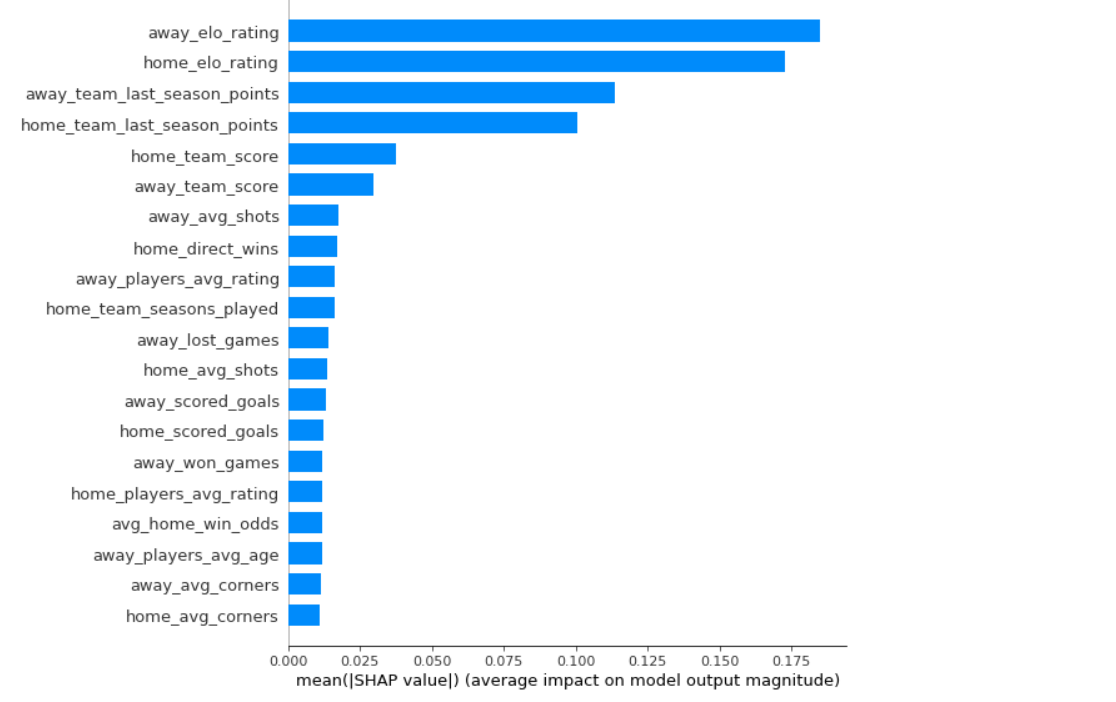
\includegraphics[width=10cm,height=6cm]{figures/ShapSVM.png}
        \caption{Wartości Shapleya dla SVM}\label{Shap-SVM}
\end{figure}
W tym przypadku, również wartości elo\_rating odgrywały kluczową rolę dla algorytmu SVM. Interpretacja może być podobna, gdyż wartość ta to zagregowana i wyliczona wartości siły i zdolności danej drużyny, czyli mająca realny wpływ na to, jak dana drużyna ma aktualnie predyspozycje oraz zdolności. Ponadto wysoką wartość przyjęły atrybuty takie jak liczba punktów danych drużyn w poprzednim sezonie oraz liczba punktów danej drużyny w aktualnie rozgrywanym sezonie. 

%Wszystkie te czynniki, oraz dobór parametrów dały rezultaty jak przedstawiono powyżej.

\section{Regresja logistyczna}
\noindent W tej sekcji przedstawione zostaną wyniki osiągnięte przez algorytm regresji logistycznej z parametrami modelu opisanymi szczegółowo w sekcji \ref{tab:params_lr}.

Testy dla algorytmu regresji logistycznej zostały przeprowadzone na kilku wersji zbiorów danych. Oprócz  oryginalnych zbiorów, rozważono pomniejszone zbiory (jak w poprzednich testach), w których pomniejszenie polegało na losowym usunięciu przykładów z klasy najbardziej licznej (\english{undersampling}). Spróbowano także wykorzystać nadlosowanie przykładów uczących metodą GlobalCS w ten sposób, że liczba obserwacji z klas najmniej licznych została wyrównana do liczby obserwacji z klasy najbardziej licznej (\english{oversampling}). Dla każdej z tej metod nauczono od podstaw algorytm klasyfikujący oraz przeprowadzono predykcję na zbiorze testowym (liczność zbioru testowego wyniosła 10\% obserwacji całego zbioru danych).

\begin{table}[H]
    \centering
    \caption{Wyliczone średnie wartości miar w różnych podejściach dla danych niezbalansowanych dla algorytmu regresji logistycznej}
    \label{tab:LRSampling}
    \begin{tabular}{| c | c | c | c | c |}
    \hline
        Podejście & Dokładność & Prezycja & Czułość & Wartość Fscore \\ \hline 
        \hline
        Oryginalny zbiór danych & 46.7\% & 44.06\% & 45.32\% & 43.95\% \\
        \hline
        \textit{Undersampling} & 52.88\% & 52.21\% & 53.16\% & 52.3\% \\
        \hline
        \textit{GlobalCS} & 45.81\% & 42.75\% & 42.74\% & 42.18\% \\
         \hline
    \end{tabular}
\end{table}

Analizując wyniki otrzymane poprzez wykorzystanie różnych podejść do problemu niezbalansowanych danych można stwierdzić, że dla algorytmu regresji logistycznej zdecydowanie najlepiej sprawdza się metoda polegająca na usunięciu obserwacji z klas bardziej licznych, która jest wykorzystana także w innych podrozdziałach.

Ponadto wykonany został kolejny test sprawdzający ile meczów wstecz dla danej drużyny powinniśmy brać pod uwagę przy wyliczaniu cech dla naszego algorytmu, tak aby maksymalizować średnie wartości dokładności, precyzji oraz czułości.

\begin{table}[H]
    \centering
    \caption{Znalezienie odpowiedniej liczby meczów dla wyliczanych cech w algorytmie regresji logistycznej}
    \begin{tabular}{| c | c | c | c | c |}
    \hline
        Liczba meczów wstecz & Dokładność & Prezycja & Czułość & Wartość Fscore \\ \hline 
        \hline
        Trzy mecze wstecz & 52.88\% & 52.21\% & 53.16\% & 52.3\% \\
        \hline
        Cztery mecze wstecz & 51.31\% & 50.97\% & 51.43\% & 50.98\% \\
        \hline
        Pięć meczów wstecz & 52.36\% & 51.71\% & 52.53\% & 51.77\% \\
         \hline
    \end{tabular}
\end{table}

Przyglądając się wynikom osiągniętym w powyższej tabeli dla dalszych testów algorytmu wykorzystany został zbiór danych, dla którego odpowiednie statystyki wyliczone są na podstawie trzech meczów wstecz.

Dokonano także przeglądu cech wykorzystywanych w algorytmie, po której to analizie zdecydowano się usunąć ze zbioru treningowego jak i uczącego cechy: \textit{home\_direct\_wins}, \textit{away\_direct\_wins}, \textit{direct\_draws}, gdyż cechy te nie dostarczały istotnych informacji algorytmowi oraz wpływały negatywnie na osiągane przez niego rezultaty. Po powyższej redukcji dokładność klasyfikacji na zbiorze testowym wyniosła 53.40\%. Poszczególne średnie wartości miary precyzji, czułości oraz wartości Fscore prezentują się następująco:

\begin{table}[H]
    \centering
    \caption{Wyliczone średnie wartości miar dla algorytmu regresji logistycznej}
    \label{tab:LRscore}
    \begin{tabular}{| c | c |}
    \hline
         Precyzja (\english{precision}) &  52.81\%\\
         \hline
         Czułość (\english{recall}) &  53.80\%\\
         \hline
         Wartość Fscore &  52.79\%\\
         \hline
    \end{tabular}
\end{table}

\newpage

Macierz pomyłek dla tego algorytmu prezentuje się następująco:

\begin{center}
\begin{table}[H]
\renewcommand{\arraystretch}{1.5}
\caption{Macierz pomyłek dla algorytmu regresji logistycznej}
\begin{center}
\begin{tabular}{|c|c|c|c|c|}
   \cline{3-5} 
   \multicolumn{1}{c}{} & & \multicolumn{3}{c|}{Predicted} \\ \cline{3-5}
   \multicolumn{1}{c}{} & & Draw & HomeWin & AwayWin \\ \hline
   
   {Observed/actual}
   & Draw & 23 & 18 & 24 \\ \cline{2-5}
   & HomeWin & 10 & 40 & 9  \\ \cline{2-5}
   & AwayWin & 15 & 13 & 39 \\ \hline
\end{tabular}
\end{center}
\end{table}
\end{center}

Na podstawie powyższych wyników można wyciągnąć podobne wnioski jak we dwóch wcześniejszych podejściach. Algorytm zdecydowanie radził sobie najgorzej z typowaniem remisów w przeciwieństwie do typowania zwycięstwa którejś z drużyn. \\

Ważność odpowiednich cech dla algorytmu została ustalona poprzez wykorzystanie metody \textit{coef\_} dla modelu regresji logistycznej z biblioteki \textit{scikit-learn}. Wartości z poniższej tabeli należy odpowiednio interpretować: im wyższa wartość współczynnika dla danej cechy tym ta cecha odgrywała większą rolę w procesie predykcji ostatecznej klasy dla danej obserwacji. Analogicznie im mniejsza wartość współczynnika tym ważność danej cechy w całym procesie była mniejsza. Tabela zbierająca ważności cech prezentuje się następująco:

\begin{table}[H]
        \caption{Ważność cech modelu regresji logistycznej}
        \centering
        \begin{tabular}{c c c}
        \toprule
            Cecha & Współczynnik \\
        \midrule
            avg\_away\_win\_odds & 0.0232 \\
            home\_avg\_shots & 0.0215 \\
            avg\_home\_win\_odds & 0.0203 \\
            home\_scored\_goals & 0.0198 \\
            away\_avg\_shots & 0.0166 \\
            away\_players\_avg\_age & 0.016 \\
            home\_players\_avg\_rating & 0.0159 \\
            away\_players\_avg\_rating & 0.0148 \\
            home\_team\_seasons\_played & 0.0147 \\
            away\_won\_games & 0.0108 \\
            away\_avg\_corners & 0.0105 \\
            avg\_draw\_odds & 0.0097 \\
            home\_avg\_corners & 0.0077 \\
            away\_lost\_games & 0.0073 \\
            away\_tied\_games & 0.0064 \\
            away\_scored\_goals & 0.0063 \\
            home\_tied\_games & 0.0039 \\
            away\_team\_score & 0.0039 \\
            home\_players\_avg\_age & 0.0038 \\
            away\_team\_seasons\_played & 0.0034 \\
            home\_team\_score & 0.0033 \\
            away\_team\_last\_season\_points & 0.0021 \\
            home\_lost\_games & 0.0019 \\
            home\_elo\_rating & 0.0019 \\
            away\_elo\_rating & 0.0014 \\
            home\_team\_last\_season\_points & 0.0009 \\
            home\_won\_games & 0.0008 \\
        \bottomrule
        \end{tabular}
        \end{table}

Na podstawie powyższej tabeli można zauważyć, że najwyższy wpływ na dokonaną predykcję mają wartości kursów oferowanych przez zakłady bukmacherskie. Zdawano sobie sprawę, że te atrybuty mogą mieć znaczenie w problemie predykcji wyniku meczu, dlatego nie jest to rezultat zaskakujący. Warto także podkreślić wartości dla cech związanych z liczbą strzałów oraz liczbą zdobytych goli w ostatnich meczach. W przeciwieństwie do poprzednich modeli cechy związane z elo\_ratingiem są nisko klasyfikowane, praktycznie znajdują się na końcu tej listy, co może być pewnym zaskoczeniem. Na podstawie wartości otrzymanych dla cech powiązanych z elo\_ratingiem można wyciągnąć wniosek, że algorytm regresji uznał te cechy za mniej ważne w procesie predykcji na rzecz cech związanych z kursami bukmacherskimi, liczbą strzałów czy ogólną średnią drużyny wyliczoną na podstawie statystyk z gry FIFA.

\section{Las losowy}
\label{resultsRF}
\noindent Sekcja przedstawia  wyniki osiągnięte przez algorytm lasu losowego. Postępowanie w procesie treningu modelu odbyło się analogicznie jak przy algorytmie regresji logistycznej. Dla każdego z trzech wcześniej opisanych podejść: uczenie na oryginalnym zbiorze danych, uczenie na pomniejszonym zbiorze danych oraz uczenie na powiększonym zbiorze danych dokonano procesu nauki od podstaw algorytmu klasyfikującego oraz przeprowadzono predykcję na zbiorze testowym (liczność zbioru testowego wyniosła 10\% obserwacji całego zbioru danych), która pozwoliła na ostateczny wybór wykorzystanego podejścia.

\begin{table}[H]
    \centering
    \caption{Wyliczone średnie wartości miar w podejściu dla danych niezbalansowanych dla algorytmu lasu losowego}
    \label{tab:LRSampling}
    \begin{tabular}{| c | c | c | c | c |}
    \hline
        Podejście & Dokładność & Prezycja & Czułość & Wartość Fscore \\ \hline 
        \hline
        Oryginalny zbiór danych & 50.66\% & 52.1\% & 45.54\% & 41.02\% \\
        \hline
        \textit{Undersampling} & 49.21\% & 48.16\% & 49.22\% & 48.23\% \\
        \hline
        \textit{GlobalCS} & 49.78\% & 44.89\% & 45.59\% & 43.47\% \\
         \hline
    \end{tabular}
\end{table}

Jak można zauważyć na podstawie powyższej tabeli wyniki dla trzech różnych podejść okazały się bardziej zbliżone aniżeli to było w przypadku wcześniej omówionych modeli. Do dalszego testowania zdecydowano się wykorzystać podejście opierające się na wykorzystaniu w procesie uczenia oryginalnego zbioru danych, gdyż cechowało ono się najwyższą wartością dokładności oraz precyzji, choć czułość jest slabsza. Wybór ten zostanie także uargumentowany w dalszej części pracy.

Kolejno, podobnie jak we wcześniejszym algorytmie, zdecydowano się zbadać parametr odpowiadający za liczbę meczów wstecz, na podstawie której są wyliczane odpowiednie atrybuty dla przedstawianych algorytmów.

\begin{table}[H]
    \centering
    \caption{Znalezienie odpowiedniej liczby meczów dla wyliczanych cech w algorytmie lasu losowego}
    \begin{tabular}{| c | c | c | c | c |}
    \hline
        Liczba meczów wstecz & Dokładność & Prezycja & Czułość & Wartość Fscore \\ \hline 
        \hline
        Trzy mecze wstecz & 50.66\% & 52.1\% & 45.54\% & 41.02\% \\
        \hline
        Cztery mecze wstecz & 47.58\% & 31.17\% & 41.4\% & 34.78\% \\
        \hline
        Pięć meczów wstecz & 47.14\% & 30.97\% & 41.06\% & 34.53\% \\
         \hline
    \end{tabular}
\end{table}

Na podstawie powyższych wyników można jednoznacznie stwierdzić, że cechy obliczane na podstawie trzech meczów wstecz dla danej drużyny, zdecydowanie najlepiej współpracują z algorytmem lasu losowego. Wartości w każdej kolumnie wierszu pierwszego tabeli są wyższe aniżeli wartości z pozostałych wierszy tabeli. Badanie to ukierunkowuje nas na jednoznaczny wybór tego parametru w dalszej analizie problemu.

Dla algorytmu lasu losowego także zdecydowano przeprowadzić się selekcję cech - próbowano usunąć ze zbioru danych atrybuty odznaczające się najmniejszym wpływem w procesie wyboru ostatecznej klasy dla danej obserwacji, jednak każda taka operacja skutkowała pogorszeniem wartości na przedstawianych metrykach. Ostatecznie zdecydowano się pozostawić wszystkie cechy w zbiorze danych. Algorytm lasu losowego poprzez losowy wybór podzbioru atrybutów w procesie podziału w węźle sam potrafi wyselekcjonować najbardziej pożądane cechy w procesie uczenia, co zostało dokładniej opisane w sekcji \ref{algRandomForest}.

Po przeprowadzonym procesie uczenia i tuningu algorytmu otrzymano następujące wyniki dla przedstawianego algorytmu. Wartość dokładności zmierzona na zbiorze testowym wyniosła 50.66\%. Poszczególne miary precyzji, czułości oraz wartości Fscore przedstawione zostały w tabeli \ref{tab:RFScore}.

\begin{table}[H]
    \centering
    \caption{Wyliczone średnie wartości miar dla algorytmu lasu loswego}
    \label{tab:RFScore}
    \begin{tabular}{| c | c |}
    \hline
         Precyzja (\english{precision}) &  52.1\%\\
         \hline
         Czułość (\english{recall}) &  45.54\%\\
         \hline
         Wartość Fscore &  41.02\%\\
         \hline
    \end{tabular}
\end{table}

Macierz pomyłek dla tego algorytmu prezentuje się następująco:

\begin{center}
\begin{table}[H]
\renewcommand{\arraystretch}{1.5}
\caption{Macierz pomyłek dla algorytmu lasu losowego}
\begin{center}
\begin{tabular}{|c|c|c|c|c|}
   \cline{3-5} 
   \multicolumn{1}{c}{} & & \multicolumn{3}{c|}{Predicted} \\ \cline{3-5}
   \multicolumn{1}{c}{} & & Draw & HomeWin & AwayWin \\ \hline
   
   {Observed/actual}
   & Draw & 4 & 42 & 18 \\ \cline{2-5}
   & HomeWin & 1 & 78 & 19  \\ \cline{2-5}
   & AwayWin & 2 & 30 & 33 \\ \hline
\end{tabular}
\end{center}
\end{table}
\end{center}

To co może się rzucać na pierwszy rzut oka to fakt, że algorytm lasu losowego ma bardzo małą skuteczność w porównaniu do poprzednich algorytmów w rozpoznaniu klasy remisów. Z tego względu zdecydowano się także pokazać proces uczenia na oryginalnym zbiorze danych aniżeli na zbiorze pomniejszonym lub powiększonym o kolejne obserwacje. W tym przypadku doszło do sytuacji opisywanej w podrozdziale \ref{ImbalancedData}. Dla opisywanego algorytmu działaliśmy na danych niezbalansowanych: liczba obserwacji, w których mecz wygrała drużyna grająca na swoim stadionie wyniosła 1021, liczba obserwacji, w których mecz wygrała drużyna grająca na wyjeździe wyniosła 662, liczba obserwacji, w których odnotowano remis w meczu wyniosła 586. W tym przypadku doszło do faworyzowania przez wyuczony klasyfikator klasy dominującej kosztem klasy zdominowanej. Na podstawie macierzy pomyłek możemy zaobserwować, że algorytm przydzielił etykietę ,,HomeWin'' aż 150 obserwacjom ze zbioru 227 przykładów, co stanowi ponad 66\% całego zbioru testowego. W tym przypadku model mimo wysokich wartości dokładności i precyzji nie poradził sobie zbyt dobrze z predykcją etykiet końcowych.


Dla omawianego modelu można jeszcze dokonać spojrzenia na ważność cech modelu, które przyczyniły najbardziej się do predykcji konkretnego wyniku. Do przedstawienia ważności cech wykorzystano metodę \textit{feature\_importances\_} z biblioteki scikit-learn.

\begin{table}[H]
        \caption{Ważność cech modelu lasu losowego}
        \centering
        \begin{tabular}{c c c}
        \toprule
            Cecha & Ważność \\
        \midrule
            avg\_home\_win\_odds & 0.1321 \\
            avg\_away\_win\_odds & 0.1288 \\
            home\_players\_avg\_rating & 0.085 \\
            home\_elo\_rating & 0.0822 \\
            avg\_draw\_odds & 0.0765 \\
            home\_team\_last\_season\_points & 0.0576 \\
            away\_players\_avg\_rating & 0.054 \\
            away\_elo\_rating & 0.0493 \\
            away\_team\_last\_season\_points & 0.033 \\
            away\_players\_avg\_age & 0.0296 \\
            home\_avg\_shots & 0.0266 \\
            home\_avg\_corners & 0.0262 \\
            away\_avg\_shots & 0.0211 \\
            away\_direct\_wins & 0.02 \\
            home\_players\_avg\_age & 0.02 \\
            home\_scored\_goals & 0.0187 \\
            away\_team\_score & 0.0171 \\
            home\_team\_score & 0.0162 \\
            away\_avg\_corners & 0.0151 \\
            away\_scored\_goals & 0.0139 \\
            home\_direct\_wins & 0.0135 \\
            home\_team\_seasons\_played & 0.0112 \\
            away\_team\_seasons\_played & 0.0092 \\
            home\_tied\_games & 0.0075 \\
            direct\_draws & 0.0074 \\
            home\_won\_games & 0.0068 \\
            away\_lost\_games & 0.0064 \\
            away\_won\_games & 0.0059 \\
            home\_lost\_games & 0.0053 \\
            away\_tied\_games & 0.0037 \\
        \bottomrule
        \end{tabular}
\end{table}

Na podstawie powyższej tabeli można zauważyć wysokie znaczenie cech związanych z kursami bukmacherskimi oraz wartością elo\_rating - pokrywa się to z wcześniejszymi wnioskami oraz najważniejszymi cechami, które były przedstawiane przy okazji poprzednich algorytmów. Wysoką ważność ma także zagregowana siła drużyny na podstawie statystyk zawodników z gry FIFA, co może sugerować, że producent dobrze odwzorował istniejącą rzeczywistość w wirtualnym świecie. Również, podobnie jak w algorytmie SNN oraz SVM, dużą ważność przyjęły atrybuty związane z liczbą punktów zdobytych przez daną drużynę w poprzednim sezonie.

\section{Multi-class Rougly Balanced Bagging}
\noindent Sekcja ta stanowi rozszerzenie do sekcji \ref{resultsRF}, w której przedstawiono wyniki modelu lasu losowego na oryginalnym zbiorze danych. Po analizie rezultatów można było dojść do wniosku, że algorytm ten nie radzi sobie zbyt dobrze z problemem danych niezbalansowanych. W celu poprawy tego podejścia zdecydowano przetestować algorytm Multi-class Roughly Balanced Bagging (dalej oznaczany jako MRBB), opisany w sekcji \ref{ImbalancedData}, gdzie jako jako klasyfikator bazowy wykorzystamy algorytm drzewa decyzyjnego.

Po przeprowadzonym procesie uczenia uzyskano następujące wyniki na zbiorze testowym:

\begin{table}[H]
    \centering
    \caption{Porównanie średniej wartości miar dla algorytmu lasu losowego oraz MRBB}
    \begin{tabular}{| c | c | c | c | c |}
    \hline
        Algorytm & Dokładność & Prezycja & Czułość & Wartość Fscore \\ \hline 
        \hline
        Las losowy & 50.66\% & 52.1\% & 45.54\% & 41.02\% \\
        \hline
        MRBB & 49.33\% & 47.84\% & 47.58\% & 47.31\% \\
        \hline
    \end{tabular}
\end{table}

Na podstawie powyższej tabeli możemy zauważyć, że algorytm lasu losowego odznaczał się wyższymi wartościami na kryterium dokładności oraz precyzji oraz niższymi wartościami na kryterium czułości oraz wartości Fscore. Warto spojrzeć także na porównanie macierzy pomyłek dla obu tych podejść przed wyciągnięciem wniosków. Komórka w macierzy pomyłek została zapisana w postaci: wartość komórki z macierzy pomyłek lasu losowego/wartość komórki z macierzy pomyłek algorytmu MRBB.

\begin{center}
\begin{table}[H]
\renewcommand{\arraystretch}{1.5}
\caption{Macierz pomyłek dla algorytmu lasu losowego oraz MRBB}
\begin{center}
\begin{tabular}{|c|c|c|c|c|}
   \cline{3-5} 
   \multicolumn{1}{c}{} & & \multicolumn{3}{c|}{Predicted} \\ \cline{3-5}
   \multicolumn{1}{c}{} & & Draw & HomeWin & AwayWin \\ \hline
   
   {Observed/actual}
   & Draw & 4/21 & 42/20 & 18/23 \\ \cline{2-5}
   & HomeWin & 1/17 & 78/58 & 19/23  \\ \cline{2-5}
   & AwayWin & 2/10 & 30/22 & 33/33 \\ \hline
\end{tabular}
\end{center}
\end{table}
\end{center}

Obserwując wartości odnotowane w macierzy pomyłek zauważamy, że algorytm MRBB zdecydowanie lepiej radzi sobie z przewidywaniem remisów aniżeli algorytm lasu losowego. Również widoczna jest różnica w przydziale etykiety ,,HomeWin'' dla danej obserwacji. Dla tego algorytmu przydzielono jedynie taką etykietę 90 razy, podczas gdy dla modelu lasu losowego taka sytuacja wystąpiła 150 razy. Na podstawie tych obserwacji możemy także wyciągnąć wniosek jak ważna w analizowanym problemie była umiejętność poradzenia sobie z danymi niezbalansowanymi czy to poprzez odsianie bądź dolosowanie obserwacji lub poprzez wykorzystanie rozszerzeń standardowych algorytmów dla danych niezbalansowanych.

\section{Porównanie algorytmów}

\noindent Podsumowując i porównując wszystkie metody - klasyfikatory można stwierdzić, że prowadzą one do w miarę porównywalnych dokładności predykcji (około 49--51\%). Tak jak dyskutowaliśmy, osiągnięcie dużo wyższych trafności okazało się niemożliwe ze względu na trudność samego zadania oraz specyfikę danych. Może to być przedmiotem dalszych badań naukowych. 

Porównywane klasyfikatory różnią się wartościami średnich czułości oraz precyzji oraz rozpoznawaniem poszczególnych klas. To może być przesłanką dla użytkowników -- analityków sportowych, którzy zgodnie z swoimi preferencjami mogą wybrać jeden z klasyfikatorów lub użyć je jako zespół. 

Dodatkowo warto wspomnieć, że podczas testowania algorytmów wykorzystaliśmy technikę dotyczącą przesuwnego zbioru testowego, którego ideę przedstawiono w rozdziale \ref{section:ocenaWynikow}. Technika ta została wypróbowana w sztucznych sieciach neuronowych, jednakże ze względu na niezadowalające rezultaty, nie została ona rozwinięta w odpowiedniej podsekcji. Wyniki dokładności wahały się pomiędzy $37.5\%$ do $51.5\%$ i ostatecznie, klasyfikator ten spisywał się dużo gorzej niż podczas standardowego procesu uczenia na jednokrotnym podziale na zbiór uczący vs. testowy (wtedy rozmiar zbioru uczącego jest większy).